\section{Auswertung}
\label{sec:Auswertung}

Wurde im Folgenden ein Versuch ohne Dancerarm durchgeführt, so wurde der Draht direkt über das Kugellager der darunter liegenden Leiste geführt. Des weiteren gilt für alle folgenden Graphiken, dass die Unsicherheitsbalken stets die einfache Standardabweichung angebegen.\newline


Wickelt man die selbe Wicklung, auf der Spule $SP_K$, zweimal mit unterschiedlicher Geschwindigkeit, so wird der, bereits in \autoref{sec:Physikalisches Modell} erwähnte, Effekt einer geschwindigkeitsabhängigen Drahtspannung , bzw. Rückstellkraft $F_R$ sichtbar. Der Versuch wurde je einmal mit Dancerarm und einmal ohne Dancerarm durchgeführt.

\begin{figure}[H]
    \centering
    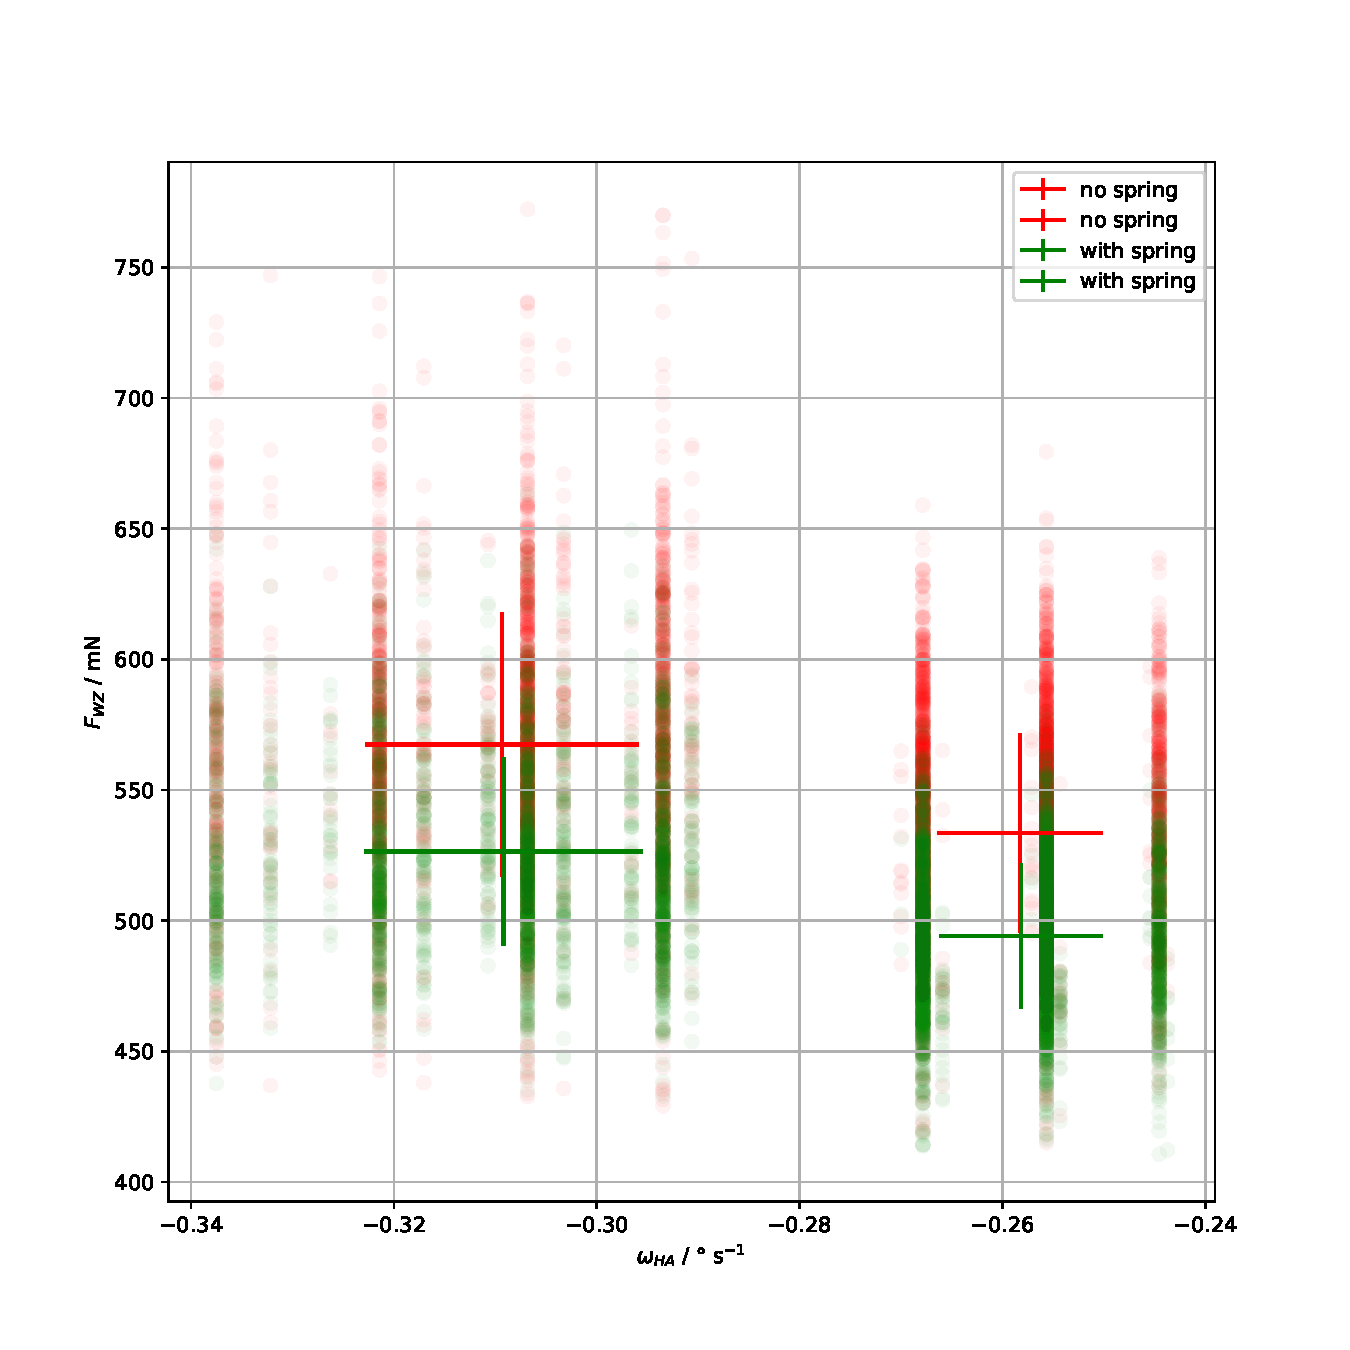
\includegraphics[width=0.9\textwidth]{./const_speed.pdf}
    \caption{Darstellung der an der Wägezelle gemessenen Kraft während einer Wickelphase mit vorgegebener, konstanter Geschwindigkeit, $F_{WZ}$ in Abhängigkeit von der Winkelgeschwindigkeit der Hauptachse $\omega_{HA}$. Die, mit Unsicherheitsbalken versehenen, vier Datenpunkte beschreiben jeweils das arithmetische Mittel des angegeben Größe.}
    \label{fig:plot_const_speed}
\end{figure}
% \begin{wrapfigure}{l}{0.6\textwidth}
%     \centering
%     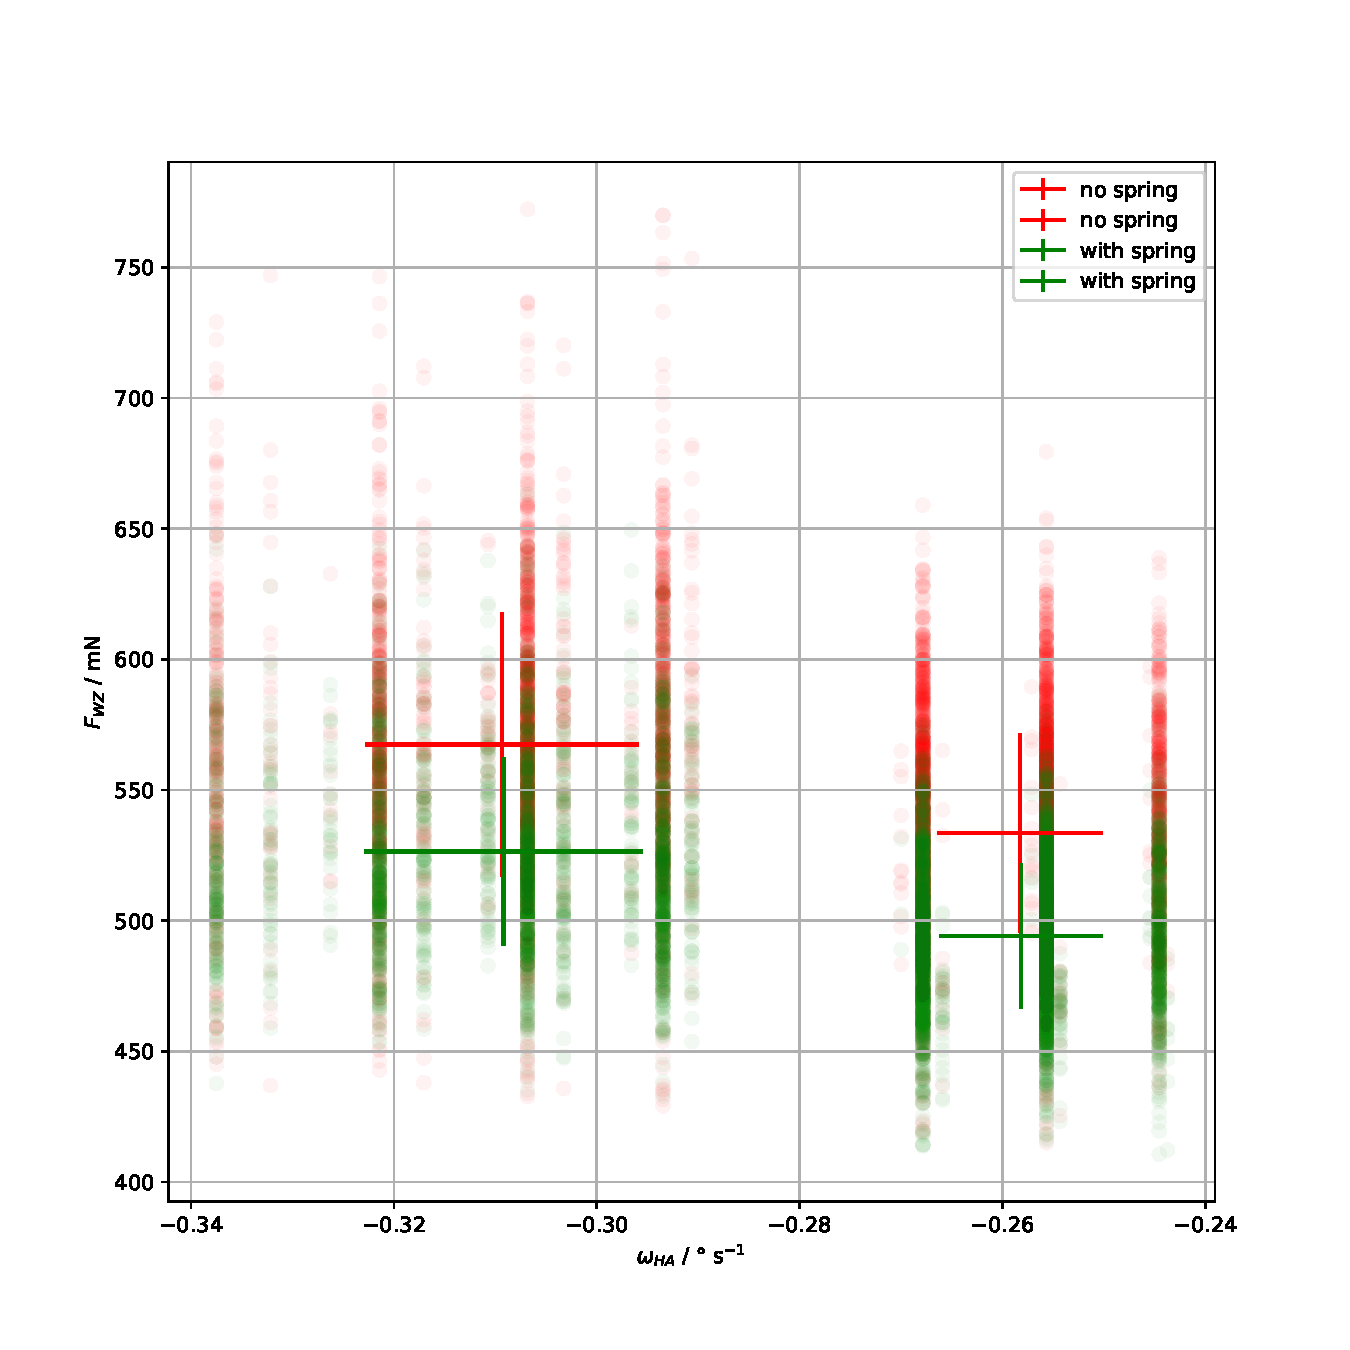
\includegraphics[width=0.6\textwidth]{./const_speed.pdf}
%     \label{fig:plot_const_speed}
% \end{wrapfigure}

Eine mögliche Erklärung für die, in siehe \autoref{fig:plot_const_speed} ersichtliche, Geschwindigkeitsabhängigkeit der Drahtspannungskraft $\tau(v)$, bzw. Rückstellkraft $F_R(v)$, wäre, dass sich die Reibung an Filz !!!!!!!!!!!!! \newline
% #TODO:Schreiben
% Einfügen erklärung filz wie gas reibung und Erklärung kugellageröl viskosität


Für den nächsten Versuch wurden die selbe Wicklung, bei gleichbleibenden Wickelparametern, einmal mit Dancerarm und einmal ohne, je für beide Spulenkörper, durchgeführt. 


% \begin{figure}[H]
%     \centering
%     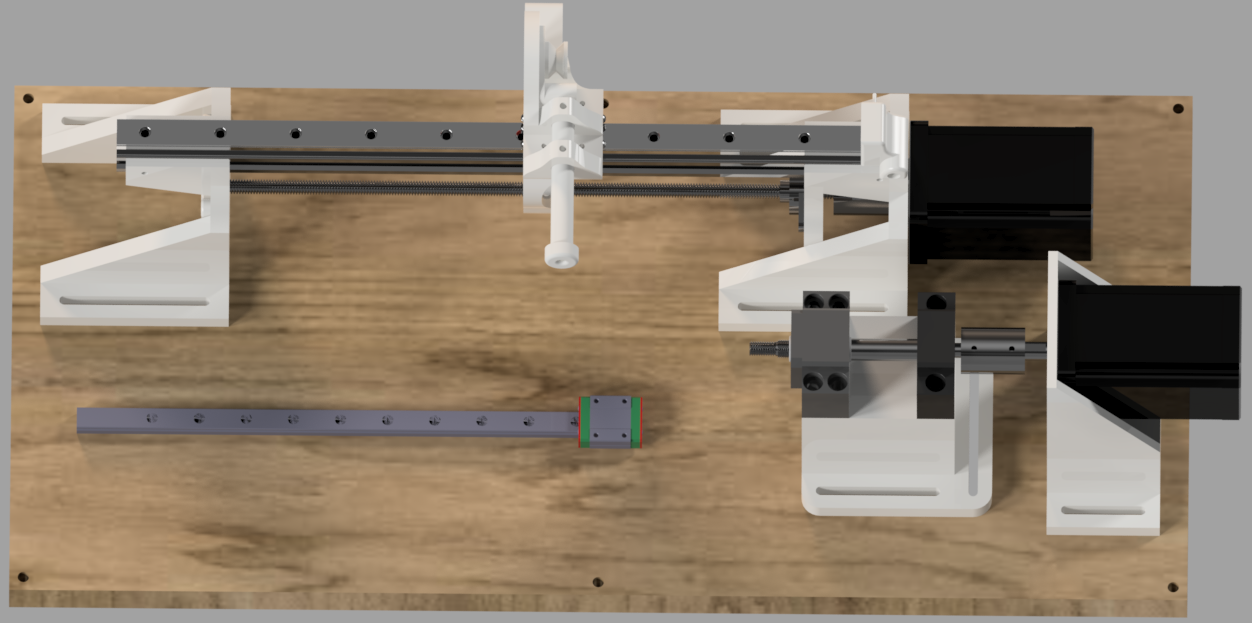
\includegraphics[width=0.25\textwidth]{./winder_render.png}
%     \caption{a nice plot}
%     \label{fig:winder_render}
% \end{figure}
% \begin{wrapfigure}{l}{0.35\textwidth}
%     \centering
%     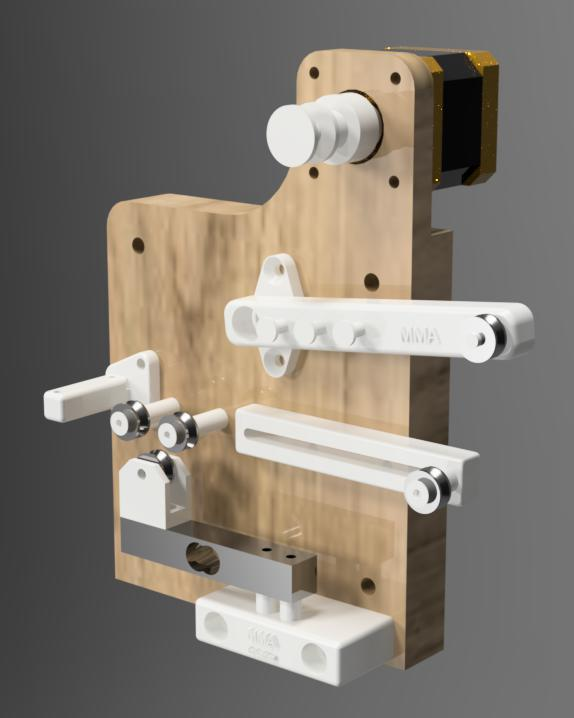
\includegraphics[width=0.35\textwidth]{./spannplatte_render.jpg}
% \end{wrapfigure}


% Text erklärung des Bildes



Zur Untersuchung der Start-, bzw. Abbremsphasen eines Wickeldurchganges sind in autoref{}!!!! die zwei Phasen, je für beide Spulentypen dargestellt. Die Messungen wurde jeweils mit der selben Beschleunigung und Endgeschwindigkeit durchgeführt.


% \begin{figure}[H]
%     \centering
%     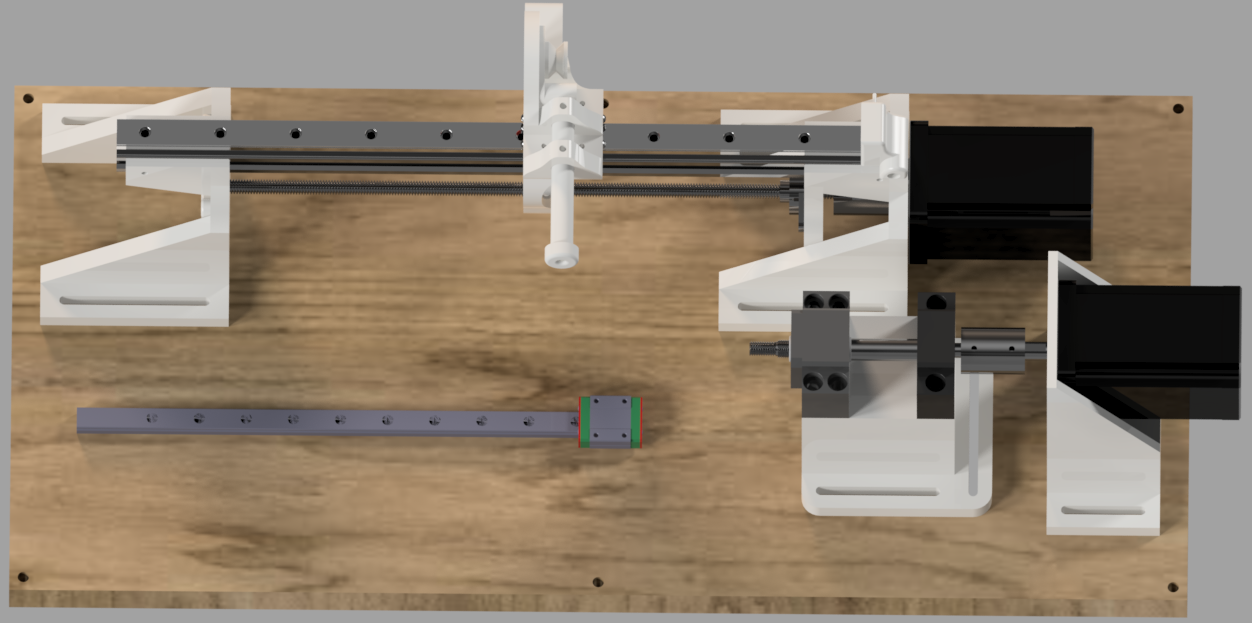
\includegraphics[width=0.25\textwidth]{./winder_render.png}
%     \caption{a nice plot}
%     \label{fig:winder_render}
% \end{figure}
% \begin{wrapfigure}{l}{0.35\textwidth}
%     \centering
%     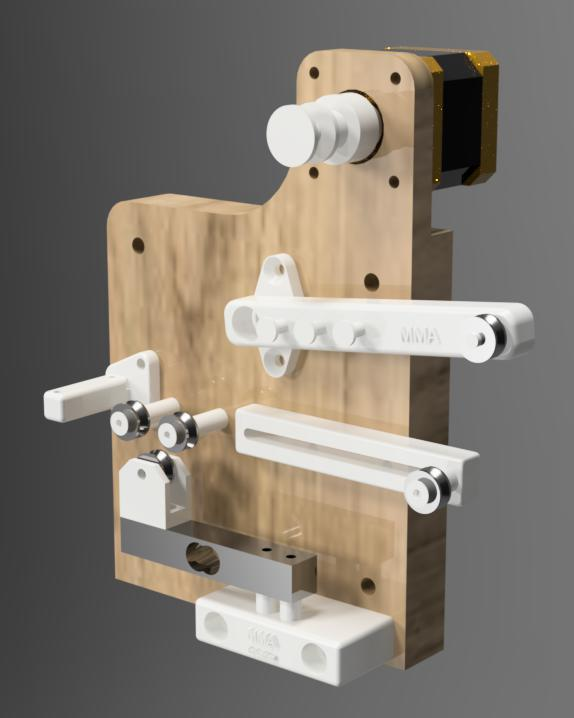
\includegraphics[width=0.35\textwidth]{./spannplatte_render.jpg}
% \end{wrapfigure}


% Text erklärung des Bildes





